\title{Bayesian Inference}

(This is just a recall of my notes on bayesian inference, because I always
forget Bayes rule.)

\section{Philosophical comment}

Consider the following sentence

\begin{quote}
\emph{The probability that tossing the coin~$X$ you get heads is~$51\%$}
\end{quote}

What does it mean, exactly?

This is an important and difficult question.  There is not a scientific
consensus about the meaning of this sentence.  There are two, very different,
answers: the so-called~\emph{frequentist} and~\emph{bayesian} interpretations
of probability.

The {\bf frequentist} interpretation is that this sentence gives a precise
information about the coin~$X$.  It says that the coin is somewhat biased
towards heads and against tails, and that if you repeat this experiment a
huge amount of times, it is very likely that you'll get more heads than
tails.  Precisely, the ratio of heads to tails will~\emph{converge}
towards~$51/49$ as the number of tosses tends to infinity.

The {\bf bayesian} interpretation is that this sentence gives a precise
information~\emph{about you}, not about the coin~$X$.  It says that your
current state of knowledge leads you to believe that it is more likely that
on the next toss, you will get heads rather than tails.  More precisely, that
if you were to place a bet on that coin toss, you would bet~$51$ against~$49$
that the result is heads.

The frequentist interpretation is a statement about the physical world, thus
it can be either true or false.  If it is true, then the sentence that the
probability of heads is~$52\%$ must be false because they are incompatible.
Also the sentence that the probability of heads is~$51.00000000001\%$, must
be false.  However, notice that it would be very, very difficult to check
which one of these sentences is true and which one is false, just by doing
experiments.  Consider that instead of tossing a coin you toss an omelette,
and that it gets destroyed after the first toss.  Can this sentence still
have a meaning?  Will you be able to ever check whether it is true or false?
I find the frequentist interpretation very difficult to understand.  Please,
somebody explain it to me more clearly.  I cannot honestly write about it
without my text looking like a straw man argument.

The bayesian interpretation is a statement about your personal beliefs, so it
does not really make sense to say that it is true or false.  Notice, in
particular, that the bayesian interpretation does not talk about the physical
world itself, only about your knowledge of this world.  The physical world
itself is deterministic.  The coin will land head or tails according to its
initial position and speed, following the deterministic laws of nature.  It
is only because you do not know with enough precision the position, speed,
and all the necessary physical details that you cannot be sure whether it
will land head or tails.

What can you do, then, with a sentence about your personal beliefs?  Can you
do science with it?  Yes, you can.  The only thing that you can do is run
experiments and update your beliefs, after looking at the results of the
experiments.  This is what bayesian inference is all about: you have some
prior beliefs and you update them using the basic laws of probability theory.

\section{Bayes Formula}

The definition of conditional probability is
$$
P(A|B)=\frac{P(A\cap B)}{P(B)}
$$
then, by simple algebraic manipulation, and using different letters, you
obtain Bayes formula:
$$
P(\theta|D)=\frac{P(D|\theta)P(\theta)}{P(D)}
$$

You can interpret this formula in the following way

\begin{itemize}
	\item[$D$] the observed data
	\item[$\theta$] the parameters
	\item[$P(\theta)$] your \emph{prior} knowledge about the parameters
	\item[$P(\theta|D)$] your knowledge about the parameters after having
		observed the data (the \emph{posterior})
	\item[$P(D|\theta)$] the ``generative model'': given a value of the
		parameters, what is the distribution distribution of the data?
	\item[$P(D)$] a normalization factor equal to~$\int\theta
		P(D|\theta)P(\theta)\mathrm{d}\theta$.
\end{itemize}

This formula tells you how to update your prior knowledge~$P(\theta)$ about
the parameters~$\theta$ after having observed the data~$D$.  For that, you
need to take into account the ``data generation model'', that describes how
likely is each datum for a given value of the parameters.

\section{Examples of inference}

The only way to understand inference is doing some simple examples.

\subsection{Inference for quiche-eaters}

Let us start with the easiest possible inference problem.

Let us suppose that an experiment produces independent samples of a normally
distributed random variable of mean~$\mu$ and standard deviation~$\sigma$.
We have observed~$N$ samples of values~$x_1,\ldots,x_N$.  What can we say
about~$\mu$ and~$\sigma$?

If you have had some exposure to~\emph{estimation theory}, you would
automatically say, we define~\emph{estimators} for the unknown parameters,
such as
$$
\hat\mu :=\frac{1}{N}\sum_{n=1}^N x_n
$$

and

$$
\hat\sigma_1 :=\sqrt{\frac{1}{N}\sum_{n=1}^N (x_n-\hat\mu)^2}
$$

or maybe

$$
\hat\sigma_2 :=\sqrt{\frac{1}{N-1}\sum_{n=1}^N (x_n-\bar\mu)^2}
$$

or even, god forbid,

$$
\hat\sigma_3 :=\sqrt{\frac{1}{N-1.5}\ \sum_{n=1}^N (x_n-\bar\mu)^2}
$$

or, if you are really fancy, you can use an~\emph{unbiased} estimator
for~$\sigma$

$$
\hat\sigma_4
:=\frac{\Gamma\left(\frac{n-1}{2}\right)}{\Gamma\left(\frac{n}{2}\right)\sqrt{2}}\ \sqrt{\sum_{n=1}^N (x_n-\bar\mu)^2}
$$

There are more unbiased estimators for~$\sigma$, this one is just an example.
Where do these fantastic formulas come from?  From rules of thumb, you invent
them, and then you prove some properties about them: such as being unbiased,
or having minimal variance, and whatnot.  This is some serious bullshit that
you should avoid as much as possible.

\subsection{How real men do inference}

Let us start again with the easiest possible inference possible: to
estimate~$\mu$ and~$\sigma$ from independent observations~$x_1,\ldots,x_N$ of
a normal random variable.  What can we do?  We can state what we do know:

(1) We know that the values~$x_1,\ldots,x_N$ are independent samples of a
random variable of type~$\mathcal{N}(\mu,\sigma)$.

(2) We do not know anything about~$\mu$

(3) We do not know anything about~$\sigma$

Well, if that is really the case, I have bad news: there's nothing to do in
that case.

\begin{quote}
	\emph{You can't do inference---or data compression---without
	making assumptions.}\newline
	--David~J.~C.~MacKay
\end{quote}

And that's it.  Bayesian inference does not simply allow you to infer
anything from raw data.  If you want to do inference, you have to begin with
some~\emph{prior knowledge} (that may be as imprecise as you want), and then,
after having observed the data, you use Bayes rule to~\emph{update} your
knowledge according to the observations.

Since your knowledge, or lack thereof, is always modelled by probability
distributions, you have to specify a prior probability
distribution for your unknown parameters~$\mu$ and~$\sigma$.  For example,
you can suppose, that~$|\mu|\le10^6$ and
that~$0\le\sigma\le10^6$.  More precisely, we assume that~$\mu$ and~$\sigma$
are independent and that they have uniform distributions in the indicated
intervals.  This is then the prior density distribution of the parameters, that
models our knowledge before observing any data:
$$
P(\mu,\sigma)=P(\mu)\cdot P(\sigma)=
\frac{1}{2\cdot10^6}\mathbf{1}_{\left[-10^6,10^6\right]}(\mu)
\cdot
\frac{1}{10^6}\mathbf{1}_{\left[0,10^6\right]}(\sigma)
$$
This is our model for the prior: a constant function on a huge rectangle of
the plane.

More interesting is the data generation model:
$$
P(x_1,\ldots,x_N|\mu,\sigma)=
\prod_{n=1}^N \frac{1}{\sqrt{2\pi\sigma}}e^{-\frac{(x_n-\mu)^2}{2\sigma^2}}
$$
this formula is the exact translation of the sentence ``the~$x_n$ are
independent, identically distributed samples of~$\mathcal{N}(\mu,\sigma)$''.
By simple manipulation, the formula above is written as
$$
P(x_1,\ldots,x_N|\mu,\sigma)=
(2\pi\sigma)^{-N/2}\exp\left(-\sum_{n=1}^N\frac{(x_n-\mu)^2}{2\sigma^2}\right)
$$

Now, Bayes rule says
$$
P(\mu,\sigma|x_1,\ldots,x_N)\propto
P(x_1,\ldots,x_N|\mu,\sigma)\cdot P(\mu,\sigma)
$$

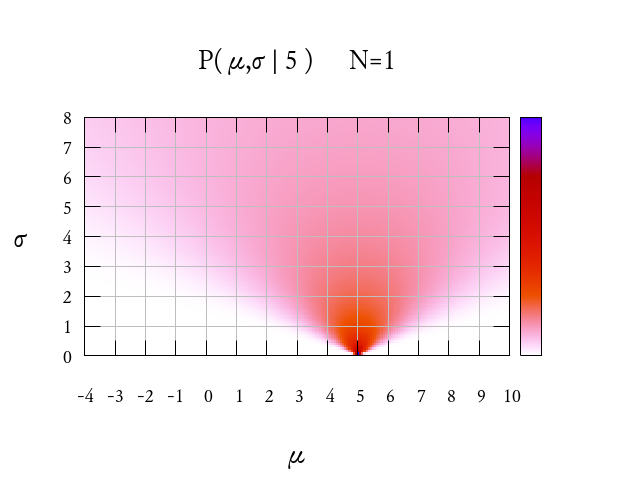
\includegraphics{bayes1.png}
%SCRIPT gnuplot <<END >bayes1.png
%SCRIPT set term pngcairo
%SCRIPT f(x,y)=exp(-((40-x)**2+(40-x)**2+(70-x)**2)/(2*y**2))/(y**(1.5))
%SCRIPT set xrange [-100:100]
%SCRIPT set yrange [0:100]
%SCRIPT set isosample 400,400
%SCRIPT set samples 200
%SCRIPT set table 'caca.dat'
%SCRIPT splot f(x,y)
%SCRIPT unset table
%SCRIPT set title "P(μ,σ|30,30,80)"
%SCRIPT set xlabel "μ"
%SCRIPT set ylabel "σ"
%SCRIPT set palette rgb 30,31,32 negative
%SCRIPT plot 'caca.dat' with image
%SCRIPT END
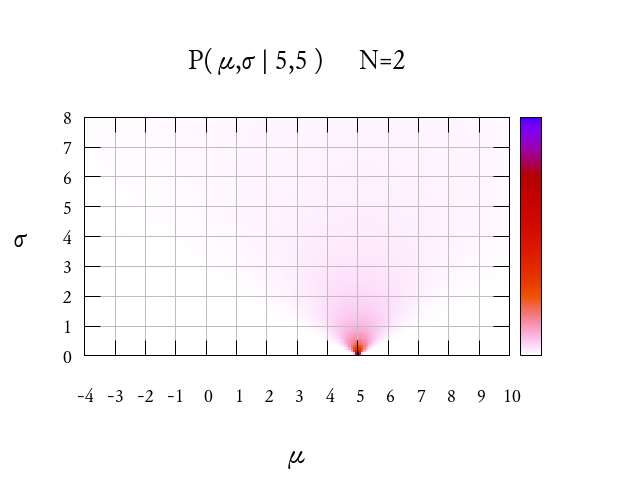
\includegraphics{bayes2.png}
%SCRIPT gnuplot <<END >bayes2.png
%SCRIPT set term pngcairo
%SCRIPT f(x,y)=exp(-((48-x)**2+(48-x)**2+(54-x)**2)/(2*y**2))/(y**(1.5))
%SCRIPT set xrange [-100:100]
%SCRIPT set yrange [0:100]
%SCRIPT set isosample 400,400
%SCRIPT set samples 200
%SCRIPT set table 'caca.dat'
%SCRIPT splot f(x,y)
%SCRIPT unset table
%SCRIPT set title "P(μ,σ|48,48,54)"
%SCRIPT set xlabel "μ"
%SCRIPT set ylabel "σ"
%SCRIPT set palette rgb 30,31,32 negative
%SCRIPT plot 'caca.dat' with image
%SCRIPT END
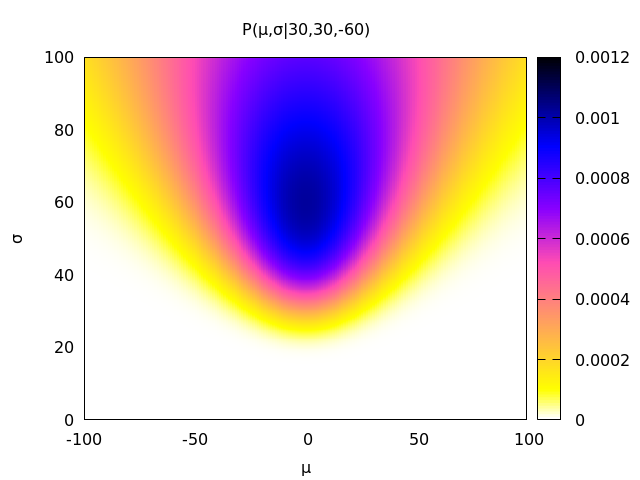
\includegraphics{bayes3.png}
%SCRIPT gnuplot <<END >bayes3.png
%SCRIPT set term pngcairo
%SCRIPT f(x,y)=exp(-((30-x)**2+(30-x)**2+(-60-x)**2)/(2*y**2))/(y**(1.5))
%SCRIPT set xrange [-100:100]
%SCRIPT set yrange [0:100]
%SCRIPT set isosample 400,400
%SCRIPT set samples 200
%SCRIPT set table 'caca.dat'
%SCRIPT splot f(x,y)
%SCRIPT unset table
%SCRIPT set title "P(μ,σ|30,30,-60)"
%SCRIPT set xlabel "μ"
%SCRIPT set ylabel "σ"
%SCRIPT set palette rgb 30,31,32 negative
%SCRIPT plot 'caca.dat' with image
%SCRIPT END
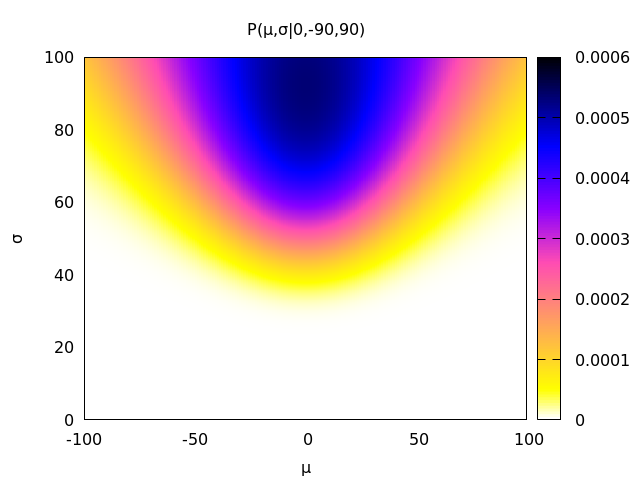
\includegraphics{bayes4.png}
%SCRIPT gnuplot <<END >bayes4.png
%SCRIPT set term pngcairo
%SCRIPT f(x,y)=exp(-((0-x)**2+(80-x)**2+(-80-x)**2)/(2*y**2))/(y**(1.5))
%SCRIPT set xrange [-100:100]
%SCRIPT set yrange [0:100]
%SCRIPT set isosample 400,400
%SCRIPT set samples 200
%SCRIPT set table 'caca.dat'
%SCRIPT splot f(x,y)
%SCRIPT unset table
%SCRIPT set title "P(μ,σ|0,-90,90)"
%SCRIPT set xlabel "μ"
%SCRIPT set ylabel "σ"
%SCRIPT set palette rgb 30,31,32 negative
%SCRIPT plot 'caca.dat' with image
%SCRIPT END





% vim:set tw=77 filetype=tex spell spelllang=en:
